\documentclass[runningheads,a4paper]{llncs}
% Springer's production compiles with pdfLaTeX; tectonic (XeTeX) builds the site copy.
\usepackage{iftex}
\ifPDFTeX
  \usepackage[T1]{fontenc}
  \usepackage[utf8]{inputenc}
  \usepackage{lmodern}
\else
  \usepackage{fontspec}
\fi
\usepackage{amsmath,amssymb}
\usepackage{microtype}
\usepackage{booktabs,array,tabularx}
\usepackage{tikz}\usetikzlibrary{arrows.meta,positioning}
\usepackage{pgfplots}\pgfplotsset{compat=1.18}
\usepackage[hidelinks]{hyperref}
\usepackage{xurl}
\newcommand{\q}[1]{«\,#1\,»}
\newcommand{\lean}[1]{\texttt{#1}}
\renewcommand{\UrlFont}{\ttfamily\small}
\setlength{\emergencystretch}{1em}

\begin{document}
\title{Formalising a Mathematician's Working Notes:\\ 2,052 Lean Theorems from the Grothendieck Archive}
\titlerunning{Formalising Grothendieck's Working Notes}
\author{Michel Hua\orcidID{0009-0002-8304-0683}}
\authorrunning{M. Hua}
\institute{Commutator, Paris, France\\ \email{michel@commutator.io}}
\maketitle

\begin{abstract}
The University of Montpellier holds the mathematical working notes of Alexandre Grothendieck, 178 openly accessible folders and some 16,000 digitised pages written between 1949 and 1991. An edition in progress has transcribed 9,414 of these pages with a large language model and restated 164 folders in current notation. This paper reports the next step: statements drawn from those restatements were formalised in Lean~4 against a pinned revision of Mathlib, in 69 files (67 folders and two Bourbaki drafts) holding 2,052 theorems that depend only on Lean's three standard axioms. We describe the pipeline from page to theorem, the rule that ties each theorem to a page without attributing to Grothendieck what the edition supplied, a triage of 203 open statements by reachability, and what the formalisation found: false glosses in the machine readings, errors on the page, statements already in print, one question of the notes answered for every~$n$ in a homogeneous model, and the relation of the work to seven conjectures that appear in the notes. We also report the reception of the general lemmas proposed to Mathlib, and the limits of human checking. A proof shows that a reading holds together; it does not show that the reading is what the page says.
\keywords{Lean \and Mathlib \and autoformalisation \and manuscripts \and language models \and Grothendieck}
\end{abstract}

\section{Introduction}

Alexandre Grothendieck gave his mathematical papers to his former student Jean Malgoire in 1990 and 1995. They were deposited at the University of Montpellier in 2010 and given to it in 2012. The university has catalogued the fonds and placed 178 folders, 16,074 pages by the inventory's count, in open access as facsimiles \cite{montpellier}. They are working notes: drafts in ink and pencil, restarted, struck and annotated, in a notation of his own. Mathematicians have edited twenty folders by hand, among them \emph{Les Dérivateurs} \cite{kmm} and the first volume of \emph{À la poursuite des champs} \cite{maltsiniotis2022}; the rest had not been transcribed.

Since August 2026 an edition has read the remaining folders with a large language model as first transcriber \cite{huajtei,repo}. By October 2026, 638 passes had read 9,414 pages in 164 folders into a restricted \LaTeX{} with a critical apparatus, and every one of the 164 folders had a \emph{modernised reading}: a restatement in current notation, in French, derived from the transcription and never from the hand. The companion paper for the \emph{Journal of the TEI} \cite{huajtei} covers the encoding of the transcriptions and the checking of the readings. This paper covers the formalisation of the statements. The rights in the manuscripts belong to Grothendieck's heirs. Following the answer of an institution consulted in September 2026, the reading views of the transcriptions are withheld from the public site until the heirs authorise them; the statements, the Lean files and the written-out proofs remain public, and each cites the page of Montpellier's facsimile.

Why formalise statements from working notes? A modernised reading is a claim that a stretch of manuscript says a particular piece of mathematics, made by a model and checked by no mathematician. The usual failures of such a reading are an inverted variance, a hypothesis the page carries and the reading drops, an inclusion turned into an equality, a modern name applied to something it does not fit. A proof assistant refuses all four. Lean cannot say whether the reading is faithful to the page, since a perfectly formalised statement can be a perfectly formalised misreading. It can say whether what the reading states holds, under which hypotheses, and with which counterexample when it does not.

The contributions are: (i) a pipeline from facsimile to Lean theorem, with a rule of attribution linking each theorem to a page (Sections~\ref{sec:pipeline} and~\ref{sec:attribution}); (ii) a triage of the open statements by what Mathlib can reach (Section~\ref{sec:triage}); (iii) an account of what the formalisation revealed about the readings and the pages, and of what it can do with the conjectures in the notes (Sections~\ref{sec:found} and~\ref{sec:conj}); (iv) a record of the reception of the derived lemmas by Mathlib, of human checking, and of costs (Sections~\ref{sec:mathlib}--\ref{sec:costs}).

\section{Corpus and Pipeline}\label{sec:pipeline}

% The pipeline from the page to the Lean theorem, and the two places a person enters.
%
% Drawn rather than generated, because it states decisions and not data.
\begin{figure}[t]\centering
\resizebox{\textwidth}{!}{%
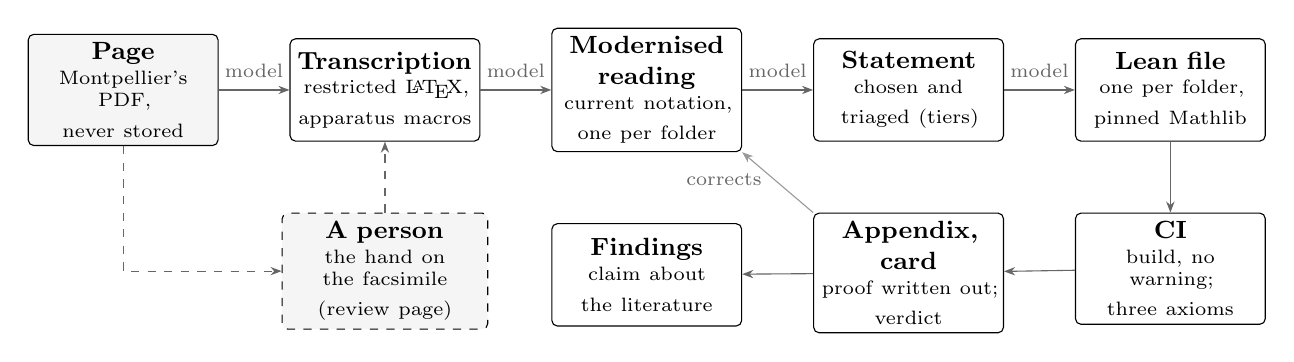
\begin{tikzpicture}[
  font=\small,
  st/.style={draw, rounded corners=2pt, align=center, inner sep=3pt,
             minimum height=13mm, text width=22mm},
  src/.style={st, fill=black!4},
  lbl/.style={font=\scriptsize, text=black!60, align=center},
  arr/.style={-{Stealth[length=4pt]}, draw=black!60},
  human/.style={arr, dashed},
]
\node[src] (P) {\textbf{Page}\\[1pt]\scriptsize Montpellier's PDF,\\\scriptsize never stored};
\node[st, right=9mm of P] (T) {\textbf{Transcription}\\[1pt]\scriptsize restricted \LaTeX,\\\scriptsize apparatus macros};
\node[st, right=9mm of T] (M) {\textbf{Modernised reading}\\[1pt]\scriptsize current notation,\\\scriptsize one per folder};
\node[st, right=9mm of M] (S) {\textbf{Statement}\\[1pt]\scriptsize chosen and\\\scriptsize triaged (tiers)};
\node[st, right=9mm of S] (L) {\textbf{Lean file}\\[1pt]\scriptsize one per folder,\\\scriptsize pinned Mathlib};
\node[st, below=9mm of L] (C) {\textbf{CI}\\[1pt]\scriptsize build, no warning;\\\scriptsize three axioms};
\node[st, below=9mm of S] (A) {\textbf{Appendix, card}\\[1pt]\scriptsize proof written out;\\\scriptsize verdict};
\node[st, below=9mm of M] (F) {\textbf{Findings}\\[1pt]\scriptsize claim about\\\scriptsize the literature};

\draw[arr] (P) -- node[lbl, above=1pt]{model} (T);
\draw[arr] (T) -- node[lbl, above=1pt]{model} (M);
\draw[arr] (M) -- node[lbl, above=1pt]{model} (S);
\draw[arr] (S) -- node[lbl, above=1pt]{model} (L);
\draw[arr] (L) -- (C);
\draw[arr] (C) -- (A);
\draw[arr] (A) -- (F);
\draw[arr, draw=black!40] (A.north west) -- node[lbl, left=1pt, pos=0.55]{corrects} (M.south east);

\node[st, dashed, fill=black!4, below=9mm of T, text width=24mm] (H)
  {\textbf{A person}\\[1pt]\scriptsize the hand on the facsimile\\\scriptsize (review page)};
\draw[human] (H.north) -- (T.south);
\draw[human] (P.south) |- (H.west);
\end{tikzpicture}}
\caption{From the page to the theorem. Every arrow marked \emph{model} is written by a language model under written rules; the dashed loop is the only place a person compares the text with the page. A failed proof or a counterexample goes back to the modernised reading (grey arrow), never to the transcription, which only a reading of the hand may change.}\label{fig:pipeline}
\end{figure}


Figure~\ref{fig:pipeline} shows the chain. The transcription is written twenty pages at a time in a \LaTeX{} subset with nine apparatus macros (illegible, uncertain, supplied, added, struck, note and the like); two scripts refuse any construct outside the subset. The modernised reading of a folder is written in one pass over all its batches, with footnotes that carry what the apparatus carried. A further register, the \emph{findings} (\texttt{src/content/findings.ts}), lists statements of the folders that may not stand in the literature, each written as a claim about the literature with what was searched and what would settle it. On 21 October 2026 it held 463 rows from 155 folders: 216 unsearched, 165 candidates, 73 matched, 8 refuted and one confirmed, a status only a person may set.

Statements are taken from the readings and the findings and formalised in \texttt{lean/Grothendieck/}, one file per folder (\lean{Folder19.lean}, \lean{Folder161\_2.lean}), plus two files, \lean{Bourbaki288.lean} and \lean{Bourbaki457.lean}, for drafts of the Bourbaki archive. Each file opens with a docstring that names the folder, the pages and what is and is not proved, and keeps its own namespace. At the commit this paper describes there are 69 files, 67 folders and the two Bourbaki drafts, with 39,562 lines and 2,052 top-level \lean{theorem} declarations (counted by \texttt{grep -c '\textasciicircum theorem'} over the committed files). The first file was committed on 26 September 2026; 185 commits have touched the directory since. The general lemmas the proofs share are kept apart, in \texttt{lean/Grothendieck/Upstream/} (Section~\ref{sec:mathlib}).

Mathlib is pinned to a revision of its \texttt{master} branch, not to a release, with the toolchain \texttt{leanprover/lean4:v4.35.0-rc4}, so that the proofs are checked against the library the derived pull requests target (Section~\ref{sec:mathlib}). Moving the pin is a deliberate step: a deprecation fails the build, and the files are rebuilt one at a time because each process importing Mathlib needs about 2\,GB. A continuous integration workflow (\texttt{.github/workflows/lean.yml}) builds the library with warnings as errors, so that a \lean{sorry} fails it, and then runs \texttt{lean/axioms.sh}. That script reads every theorem name from the files, prints \lean{\#print axioms} for each, and fails if any theorem depends on an axiom other than \lean{propext}, \lean{Classical.choice} and \lean{Quot.sound}, or if any theorem was not found. No file declares an axiom or uses \lean{native\_decide}.

\section{Attribution and the Link from Page to Theorem}\label{sec:attribution}

A formalisation of working notes must keep apart three things: what the page states, what the reading states, and what the formaliser had to add. The edition's rule is that a statement is labelled \q{Grothendieck, page~$N$} only if that page states it. A result the edition established to make a statement provable, a lemma, a weaker hypothesis that suffices, a counterexample, is given a neutral label and never his name. The same rule governs the pull requests to Mathlib: Grothendieck is named only for statements genuinely his, in one line of the description, never in a docstring.

Every proof has three human-readable forms. The Lean file is the record. A card in \texttt{src/content/proofs.ts}, rendered on the site, gives the folder, the batch and page, the reading's name for the statement, the statement, what the formalisation found, and a verdict from a closed list. The 69 cards carry these verdicts: \emph{holds} (14), \emph{holds, more generally} (16), \emph{partly proved} (33), \emph{the reading dropped a hypothesis} (3), \emph{holds; the gloss was false} (1) and \emph{false on the page} (2). The third form is an appendix in French \cite{hualean}, written for a reader who is a mathematician but not a Lean user: for each folder, the leaf in context, the statement as the reading gives it, a proof written out with its intuition, remarks, and what is not proved. Its parts follow the themes of the fonds in chronological order (Figure~\ref{fig:themes}); it runs to 277 pages. It cites the general lemmas by their file in the repository rather than proving them again. Where a formalisation bears on a finding, the finding's row records it, and a counterexample moves the row to \emph{refuted} with what still stands.

% Drawn by docs/cicm/figures.mjs on 2026-10-21 from lean/Grothendieck/*.lean at HEAD
% and the parts of docs/lean/article.tex. Do not edit by hand.
\begin{figure}[t]\centering
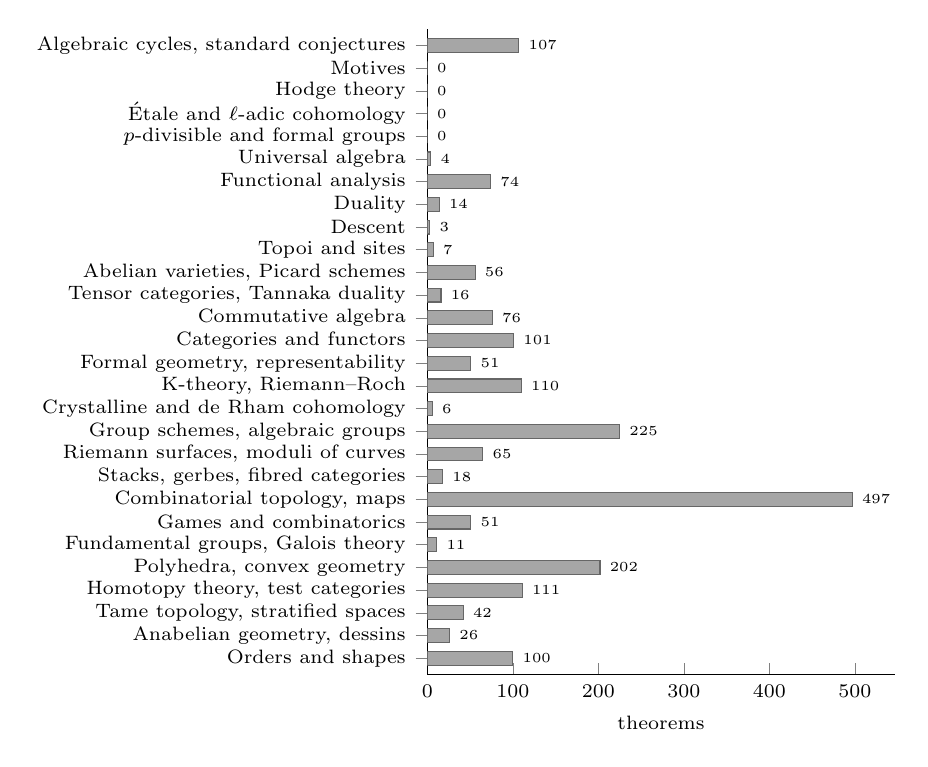
\begin{tikzpicture}
\begin{axis}[xbar, y=8.2pt, bar width=5pt, width=0.62\textwidth,
  xmin=0, enlarge y limits={abs=6pt}, xlabel={theorems}, xlabel style={font=\scriptsize},
  symbolic y coords={{Orders and shapes},{Anabelian geometry, dessins},{Tame topology, stratified spaces},{Homotopy theory, test categories},{Polyhedra, convex geometry},{Fundamental groups, Galois theory},{Games and combinatorics},{Combinatorial topology, maps},{Stacks, gerbes, fibred categories},{Riemann surfaces, moduli of curves},{Group schemes, algebraic groups},{Crystalline and de Rham cohomology},{K-theory, Riemann--Roch},{Formal geometry, representability},{Categories and functors},{Commutative algebra},{Tensor categories, Tannaka duality},{Abelian varieties, Picard schemes},{Topoi and sites},{Descent},{Duality},{Functional analysis},{Universal algebra},{$p$-divisible and formal groups},{Étale and $\ell$-adic cohomology},{Hodge theory},{Motives},{Algebraic cycles, standard conjectures}}, ytick=data,
  yticklabel style={font=\scriptsize}, xticklabel style={font=\scriptsize},
  nodes near coords, nodes near coords style={font=\tiny},
  axis x line*=bottom, axis y line*=left, every axis plot/.append style={fill=black!35, draw=black!60}]
\addplot[fill=black!35, draw=black!60] coordinates {(100,{Orders and shapes}) (26,{Anabelian geometry, dessins}) (42,{Tame topology, stratified spaces}) (111,{Homotopy theory, test categories}) (202,{Polyhedra, convex geometry}) (11,{Fundamental groups, Galois theory}) (51,{Games and combinatorics}) (497,{Combinatorial topology, maps}) (18,{Stacks, gerbes, fibred categories}) (65,{Riemann surfaces, moduli of curves}) (225,{Group schemes, algebraic groups}) (6,{Crystalline and de Rham cohomology}) (110,{K-theory, Riemann--Roch}) (51,{Formal geometry, representability}) (101,{Categories and functors}) (76,{Commutative algebra}) (16,{Tensor categories, Tannaka duality}) (56,{Abelian varieties, Picard schemes}) (7,{Topoi and sites}) (3,{Descent}) (14,{Duality}) (74,{Functional analysis}) (4,{Universal algebra}) (0,{$p$-divisible and formal groups}) (0,{Étale and $\ell$-adic cohomology}) (0,{Hodge theory}) (0,{Motives}) (107,{Algebraic cycles, standard conjectures})};
\end{axis}
\end{tikzpicture}
\caption{Lean theorems per theme, the themes being the 28 parts of the written-out appendix in their order (1973 of the 1973 theorems at HEAD; every file belongs to a part). The 4 parts at zero hold only statements left unproved. Drawn by \texttt{docs/cicm/figures.mjs} on 2026-10-21.}\label{fig:themes}
\end{figure}


\section{Triage: What Mathlib Reaches}\label{sec:triage}

The first eighteen folders were chosen by hand (issue \#26) as those whose readings would repay a proof. In October 2026 the 203 findings that were still open and had no proof, in 111 folders, were sorted by reachability (issue \#54). Tier~1, reachable now with Mathlib as it stands, held 16; tier~2, a project of a few hundred lines in which part of the statement is reachable, 39; tier~3, out of reach, 147; and one finding was ill-posed as read and set aside to be disproved. A tier says nothing about whether a statement is new.

Tier~3 is most of the corpus, and it is so for one reason: the statements live in theories that Mathlib does not yet have, or has only in foundational form. These are schemes beyond their definition and first properties, étale and $\ell$-adic cohomology, crystalline cohomology, topoi and their morphisms, stacks and gerbes, derivators, motives, and Hodge structures on cohomology. Figure~\ref{fig:themes} shows the effect. Four parts of the appendix (motives, Hodge theory, étale and $\ell$-adic cohomology, $p$-divisible groups) contain no proved statement at all, and descent only the field case of a lemma (folder 128), while combinatorial topology, polyhedra, group schemes taken in coordinates, and homotopy theory through test categories carry most of the theorems. The distribution reflects Mathlib and not the notes. Grothendieck's own centre of gravity in these folders is in the empty parts.

What can be reached is often a special case or a model. A group scheme is treated on $R$-points in coordinates over an arbitrary ring (folder 72), a statement about schemes is proved for $\operatorname{Spec} A$ with $A$ Noetherian (folder 42), a statement about a connection is proved in rank one on the trivial bundle (folder 93). Of the 69 cards, 33 say \emph{partly proved}, and each says what is not. Several others prove a statement only in a model, or in the special case that Mathlib reaches, and say so. We count such proofs as partial in spirit: a proof in a model checks that the axioms of the page are consistent and that a computation is right, not that the general statement holds. The issues that track the remaining rows (\#59, \#72) give each an estimated size and a value, and drop those whose only reachable part would be a special case of the edition's choosing.

\section{What Formalisation Revealed}\label{sec:found}

\paragraph{False glosses in the readings.} The most frequent finding is that the page is right and the reading is not, where the reading goes beyond the page. In folder 158 the Proposition holds as the leaf states it, finiteness being used exactly where the page says \q{comme $E_0$ est fini}, but the modern gloss called an element a left zero and the Rees kernel a point; in the monoid $\{1,a,b\}$ with $xa = a$ and $xb = b$ both $a$ and $b$ qualify, the kernel is $\{a,b\}$, and the element is a right zero, not unique. In folder 114 the reading dropped the page's \q{satisfying Loc~4)} from the hypotheses of a statement on fundamental localisers, without which the inclusion $W \subseteq W_0$ fails. In folder 16 the reading's universal ring $\Phi_0 = \mathbb Z[L_0, \Lambda_0]$ does not exist over $\mathbb Z$ for $n \geq 2$, since $\xi_0^n$ is divisible by $n!$; over $\mathbb Q$ the obstruction disappears. In folder 156-3 a footnote's form of the betweenness relation is false when the extremities are incomparable, as the product order on $\mathbb N^2$ shows; the lemma of the page never meets that case. Each reading was corrected. A related error was found without Lean: the summary of folder 114 had presented as true Proposition~4 of page~350 of \emph{À la poursuite des champs}, which the literature refutes by the category of cubes \cite{cisinski2006,maltsiniotis2005}.

\paragraph{Errors on the page.} Eight errors are on the page itself. In folder 19, a comonadicity theorem gives as necessary and sufficient a condition that is only sufficient: the inclusion of the pairs of sets $(X,Y)$ with $Y \neq \emptyset \Rightarrow X \neq \emptyset$ is coreflective, hence comonadic, yet fails the condition. The reading had repeated the claim and identified the condition, wrongly, with Beck's. On page~7 of the same folder the proviso \q{ou $I$ fini} is false. In folder 152 the head line of page~9 contradicts the table below it. In folder 93 a normalisation $ad - bc = 1$ added on page~121 is false, because the determinant of the homography is a unit that need not be a square ($s = 2t$ over $\mathbb F_5$). The others are an assertion that holds only under a condition written in the margin (folder 74), an index and a label carried to the wrong place (folder 86), and a translation that is wrong in characteristic~2 (folder 70). These are the slips of a man writing for himself, and they are recorded as such.

\paragraph{Statements already in print.} Formalisation often sends the edition back to the literature. In folder 16 the statement that the Lefschetz-type conjecture follows from $D(X)$ and the existence of \emph{some} algebraic isomorphism $H^{2n-i}(X) \to H^i(X)$ holds by Cayley--Hamilton in Lean. The register first listed it as possibly unpublished; it is Kleiman's Theorem~2.9 of 1968 \cite{kleiman1968}, with the same proof, and Theorem~4-1 of his 1994 survey \cite{kleiman1994}. The row is now \emph{matched}.

The comparison can also go the other way. On page~35 of folder 118 Grothendieck asks whether stability of $\mathcal W_A$ under finite products makes $A$ aspherical, and answers no with a groupoid, for which $\mathcal W_A$ is the isomorphisms. Set beside Cisinski's Proposition~4.3.2 \cite{cisinski2006}, the example shows that its condition~(g) is weaker than the others for $A = BG$, as checked in Lean in a 1-truncated model for $A = BG$; asked directly, the author confirmed that (g)~$\Rightarrow$~(c) needs a further assumption \cite{cisinskimo2026}.

\paragraph{A question of the notes settled.} Page~70 of folder 146 tabulates, for the moduli spaces $M_{0,n}$, the trivialising exponents of the line bundles $L_i$ and $L = L_1 \otimes \cdots \otimes L_n$ under the symmetric group $\mathfrak S_n$, with question marks against several entries. For $n = 4$ Lean confirms the values of the table: on $U = \mathbb P^1 \setminus \{0,1,\infty\}$ the six anharmonic substitutions act through $\mathfrak S_3$, the derivative at the moving point is a 1-cocycle whose sixth power is the coboundary of $\lambda^4(1-\lambda)^4$, and no smaller power is a coboundary; for the tensor product $L$ the exponent is the page's~3. For $n = 5$, where the page writes \q{12\,?} for both, Lean proves that $L$ has order~4 and $L_i$ order~12: the page's 12 is right for $L_i$ and not minimal for~$L$. For $n = 6$ Lean proves the orders 5 and 20, against the page's \q{20\,?} and \q{60\,?}; the trivialising functions come from exact linear algebra on the nine units of $M_{0,6}$, the lower bounds from fixed points where the factor is a primitive fifth root of unity or~$i$. The groups themselves are known: $[M_{0,n}/\mathfrak S_n]$ is the stack of smooth binary forms of degree~$n$, whose Picard group is $\mathbb Z/2(n-1)$ for $n$ even by Gorchinskiy and Viviani's Theorem~3.6 \cite{gorchinskiyviviani2008}, and the method of Arsie and Vistoli \cite{arsievistoli2004} gives the rest. For every $n$, Lean then proves the general formula in a homogeneous model, where a point of $\mathbb P^1$ is a vector of $K^2$ and a trivialisation of $L_i^{\otimes m}$ is a nowhere-zero function of weight $t^{2m}$ in the $i$-th vector and $\det(g)^m$ under $\mathrm{GL}_2(K)$, invariant under relabelling: $L$ has order $n-1$ and $L_i$ order $(n-1)(n-2)$. The trivialisations are products of brackets $[v_i\,v_j]$, a squared Vandermonde product for $L$; the lower bounds come from the configurations $\{0\} \cup \mu_{n-1}$ and $\{0,\infty\} \cup \mu_{n-2}$, rotated by $z \mapsto \omega z$. The dictionary between equivariant line bundles and these functions is not formalised. For $n$ even the order of $L_i$ is in print: Edidin and Hu, from Pernice's presentation by a Borel subgroup \cite{pernice2022}, compute the integral Chow ring of $[M_{0,2g+2}/\mathfrak S_{2g+1}]$, binary forms with a marked root, as $\mathbb Z[l]/(2g(2g+1)\,l)$ for $g \geq 2$ \cite{edidinhu2025}, and $n = 4$ follows from $\mathrm{Pic}(\mathcal M_{1,1}) = \mathbb Z/12$ \cite{mumford1965,fultonolsson2010}. What the edition adds is the odd case, which it has not found stated, and the certification in Lean.

\paragraph{A refutation outside Lean.} Bourbaki's draft no.~307 (1958) on universes asks whether there are universes other than the empty one and the $U_n$, and answers that it seems probable. Under the first definition given there, with every object in some $U_n$, the answer is no; under the second, which the text says comes to the same thing, the answer is not decided in ZFC with those axioms, since the two definitions differ at every inaccessible cardinal that is a limit of inaccessibles. The argument, which uses the classification of universes as $V_\kappa$ under foundation \cite{williams1969}, is written out in the edition's register and not formalised: Mathlib has no theory of Grothendieck universes in this form. Draft no.~288, on the exponential law for compact convergence, is formalised.

\section{Conjectures in the Notes}\label{sec:conj}

A reading of the whole fonds shows seven well-known conjectures, some earlier than the texts usually cited for them (Table~\ref{tab:conj}). The edition makes no claim of priority: a conjecture on a leaf says when he wrote it down, not that nobody had.

\begin{table}[t]\centering\scriptsize
\caption{Seven conjectures in the fonds, from the edition's note on conjectures. Dates are of the leaves or of the inventory, whose brackets mark an inferred date. The last column says whether Mathlib can state the conjecture today.}\label{tab:conj}
\begin{tabularx}{\textwidth}{@{}>{\raggedright}p{2.5cm}>{\raggedright}p{3.1cm}>{\raggedright}X>{\raggedright\arraybackslash}p{2.2cm}@{}}\toprule
Conjecture & First in the fonds & Published source & Statable in Mathlib\\\midrule
Standard conjectures & 14, p.~44, letter to Serre, 27 Aug.\ 1965 & Grothendieck 1969; Kleiman 1968, 1994 \cite{kleiman1968,kleiman1994} & no Weil cohomology\\
Period conjecture (de Rham--Betti) & 13, pp.~47--48 (1965) & Grothendieck 1966; Bost--Charles 2016 & elliptic case\\
Generalised Hodge (\(\ell\)-adic form) & 12, pp.~2--3 (1964--[c.~1971]) & Grothendieck 1969 & no\\
$p$-curvature & 93, pp.~193--197 ([1972]--1981) & Katz 1970, 1972 \cite{katz1970,katz1972} & rank one only\\
Homotopy hypothesis & 134-2, p.~42, letter to Breen, 5 Feb.\ 1975 & \emph{Pursuing Stacks} (1983) & partly\\
Galois action, $\widehat{GT}$ & 142 ([from 1978]); 119, 147 & \emph{Esquisse} (1984, publ.\ 1997) & partly\\
Section conjecture & 149, p.~65 (undated) & letter to Faltings, 1983 & no étale $\pi_1$\\\bottomrule
\end{tabularx}
\end{table}

None of the seven was in Google DeepMind's \emph{Formal Conjectures} repository \cite{formalconjectures} when the edition searched it on 17 October 2026. That repository collects open conjectures stated in Lean with a published source, and the edition's note on conjectures was posted on the Lean community's channel for it. Four of the seven cannot be stated in Mathlib today, because the objects they speak of do not exist there: a Weil cohomology theory, Hodge structures on the cohomology of a variety, the étale fundamental group. Stating such a conjecture faithfully needs those definitions first, and a statement written with ad hoc substitutes would be a different conjecture. What can be done is to prove the parts around a conjecture that rest on existing theories, and to state the conjecture in prose beside them.

Folder 93 shows the method. Pages 193--194 make a remark and ask a question. If a connection defined over the integers has finite monodromy, its reductions modulo~$p$ have vanishing $p$-curvature for almost all~$p$; is the converse true? That converse is the Grothendieck--Katz $p$-curvature conjecture. Lean proves, over a commutative ring of characteristic~$p$ with a derivation $D$, that $D^p$ is again a derivation, Jacobson's formula for the $p$-th power of $D + \mu_a$, and the easy direction in rank one on the trivial bundle: a connection trivialised by a unit has vanishing $p$-curvature. The appendix then states the conjecture in full, with its known cases, Katz's for Gauss--Manin connections \cite{katz1972}, and the solvable case through Bost and others \cite{bost2001}, and says that Lean does not touch the general case. Around the Galois action on Teichmüller towers, Lean proves the lemma of page~22 of folder 140-1, that the $\mathfrak S_3$-equivariant Picard group of $M_{0,3}$, $H^1(U_{0,3}, \mathfrak S_3; \mathbb G_m)$, is $\mathbb Z/6$, and the $n = 4$ entries of folder 146 above. Around the standard conjectures, the Kleiman match of folder 16 is formal; the step of the same folder that splits the critical-dimension condition $A^0$ into two one-sided restriction conditions $A'^0$ and $A''^0$ was not found in Kleiman's 1968 paper and stays a candidate.

The notes also pose questions with no printed source known to the edition, such as a description of the graph of the 27 lines on a cubic surface around a marked triangle as a torsor under a Baer product of quaternion extensions (folder 69), or a bound on the cohomological dimension of affine schemes of mixed characteristic, with residue characteristic~$\ell$, by the degree of imperfection (folder 31). For the latter the local form, on an open of a henselian local domain, holds in a sharper form by Gabber and Orgogozo \cite{gabberorgogozo2008}; the global bound with its \q{${}+3$} was not found in print. They cannot enter \emph{Formal Conjectures} as they stand, since that repository asks for a published source. For folder 69 the group-theoretic part is in Lean: the automorphisms preserving a triangle form a group of order $1152$, checked through a stabiliser chain.

\section{Upstreaming to Mathlib}\label{sec:mathlib}

General lemmas that the proofs needed, and that Mathlib lacked, were proposed to it as pull requests from the author's account: 41 between 10 and 20 October 2026. Not all come from this edition: the tracking issue (\#52) records some from a separate exercise in learning Lean. Those from the edition include the (co)monadicity theorem stated as an equivalence (folder 19), additive functors on the Karoubi envelope (113), fixed points of idempotent adjunctions (161-1), stable range one for semilocal rings (79), the Cauchy--Binet formula for exterior powers (1), and right zeros in finite monoids (158). Thirty-nine of the 41 carried the label that Mathlib asks for on LLM-generated contributions.

None was merged. Most were closed by Mathlib's triage account with a standard message saying that they did not meet the community's standards for the use of AI \cite{mathlibai} and that reviewer time is given first to people who can learn through review. Two, on direct categories and on the semi-simplex category, were closed after Joël Riou wrote that the first would need significant work to provide a good API, that the second took the wrong approach (a Reedy structure on the semi-simplex category should be restricted from one on the full simplex category), and that he was not enthusiastic about reviewing AI-generated pull requests. Before the closures, Eric Wieser reviewed the pull request on the symmetric Pascal matrix and asked that auxiliary facts be stated as theorems, which was done.

The lesson drawn is narrow. A lemma proved for a folder is shaped by the folder, and Mathlib wants an API, the general form, the right generality and names. A model can produce a correct proof faster than a reviewer can read it, and the community has said that it does not want to spend review on contributions whose author will not learn from the review. The lemmas now live in the repository, in 26 files under \texttt{lean/Grothendieck/Upstream/} that the proofs import, and a roadmap proposed to the Tau Ceti project specifies them for contributors who write them to Mathlib's conventions. A pull request to Mathlib is opened only after the lemma has been checked against those conventions, and new theories are discussed on Zulip first.

\section{Human Checking and Its Limits}\label{sec:checking}

The formalisation checks the readings, not the transcriptions, and not the link between them. The transcriptions are checked by spot. A page of the site, \texttt{/review/}, turns the edition's checklist into single questions, each on one spot of one page, shown beside Montpellier's facsimile with a fixed set of answers; answers come back as issues in the repository and are applied at source, with a dated revision line. By 23 October 2026 nineteen such issues had settled 173 items: 74 readings of words were changed or confirmed, 40 of them insertions whose hand was in question, and 57 dates were checked on their leaves. In all, the author has checked 135 readings against the facsimile, in 54 folders. No batch has been read whole by a person.

One answer set shows the limit. In issue \#69 the reader, who reads the hand, answered \q{can't tell} to the items that asked whether one of the edition's own arguments holds or whether a reference cited from memory is right, and most of the confirmations given earlier on such items were withdrawn. A reader of the hand is not a reader of the mathematics. A Lean proof covers part of the second need, for the statements it formalises. For the faithfulness of a statement to its page, and for everything in tier~3, the edition has no check but a specialist's, and labels its machine second readings as such.

\section{Costs and Reproducibility}\label{sec:costs}

The repository records costs in shares of a weekly usage allowance of the author's subscription, not in tokens or currency, and only for some work. A second transcription pass costs about 1\% of a week per twenty-page batch (issue \#51), and twenty-one batches of Quillen's notebooks were estimated at about 10\% (\#42). For the Lean work no cost per proof is recorded. Its scale is visible in the history: 186 commits from 26 September to 23 October, issue estimates of 80 to more than 1,200 lines per finding (\#54, \#72), and rows dropped when the estimate grew beyond their value. The constraint in practice was the weekly allowance, which bounded how many proofs ran in parallel. The code and the site are released under CC0, the Lean files build with \texttt{lake exe cache get \&\& lake build} on the pinned revision, and \texttt{axioms.sh} re-runs the axiom check.

\section{Related Work}\label{sec:related}

Mathlib \cite{mathlib2020} on Lean~4 \cite{lean4} is the library everything here depends on. Large formalisations led by mathematicians, the Kepler conjecture \cite{hales2017}, the Liquid Tensor Experiment \cite{scholze2022,castelvecchi2021} and the Fermat's Last Theorem project \cite{fltproject,best2023}, formalise a known proof towards a stated theorem. This edition goes the other way: it starts from statements scattered through drafts and asks which of them can be checked at all. Formal Abstracts \cite{formalabstracts} proposed to state the main results of published papers formally without their proofs; Formal Conjectures \cite{formalconjectures} does this for open problems with a published source. The statements here have no published source of their own, which is why the attribution rule of Section~\ref{sec:attribution} is needed.

Autoformalisation was set as a goal by Szegedy \cite{szegedy2020}. Wu et al.\ \cite{wu2022} showed that large language models can translate competition problems into formal statements, ProofNet \cite{azerbayev2023} gave a benchmark at undergraduate level, and DeepSeek-Prover \cite{xin2024} trained provers on synthetic formal data. These works measure translation and proof on curated statements. Here the statements come from manuscripts read by a model, so a failure can lie in the transcription, the reading, the formal statement or the mathematics, and only the last two are within Lean's reach.

Mathematicians' Nachlässe have been edited by hand, as the \emph{Correspondance Grothendieck--Serre} \cite{colmez2001}, \emph{Les Dérivateurs} \cite{kmm} and \emph{À la poursuite des champs} \cite{maltsiniotis2022} were. The edition's transcription method and its encoding in TEI are reported separately \cite{huajtei}.

\section{Limits and Future Work}\label{sec:limits}

Most of the open statements are out of reach until Mathlib has the theories they speak of, and the edition will not replace them by special cases of its own choosing. The rights hold means that the reading views of the transcriptions are not public, so a reader can check a theorem against the facsimile only through the statement and page reference that each card gives. The 879 drawings that the transcriptions describe in prose (issue \#73) are not yet encoded, and some statements depend on them. The tooling, built for this fonds and reused for two other archives, could become a generic tool for editing mathematical manuscripts into a checked edition (issue \#79). The checks still missing are a specialist's reading of each formal statement against its page, and of the edition's own arguments.

\section*{Declaration on the Use of Generative AI}

During the preparation of this work the author used Claude Opus~5 and Claude Opus~5.5 (Anthropic), through Claude Code, in order to transcribe the pages of the fonds, to write the modernised readings and the findings, to write the Lean proofs, the appendix and the scripts described in Sections~\ref{sec:pipeline}--\ref{sec:costs}, to prepare the pull requests to Mathlib, and to draft this paper from the repository's files and history under the author's direction. The author chose the folders and the statements to formalise, set the editorial and attribution rules, checked readings against the facsimile where the paper says so, and decided what to publish. After using these tools, the author reviewed and edited the content as needed and takes full responsibility for the content of the publication. Lean checks the proofs mechanically; the transcriptions have not been checked against the facsimiles in full by a person, and the paper says so wherever a claim depends on them.

\bibliographystyle{splncs04}
\bibliography{references}
\end{document}
